\newcommand{\figureSPI}[1]{
  \def\lang{\detokenize{#1}}
  \def\langRu{\detokenize{ru}}
  \def\langEn{\detokenize{en}}
  \def\figureCaption{XXX: No translation.}
  \ifx \lang\langRu
  \def\figureCaption{
    Шина SPI.
  }
  \fi
  \ifx \lang\langEn
  \def\figureCaption{
    SPI bus.
  }
  \fi
  \begin{figure}[ht]
    \centering
    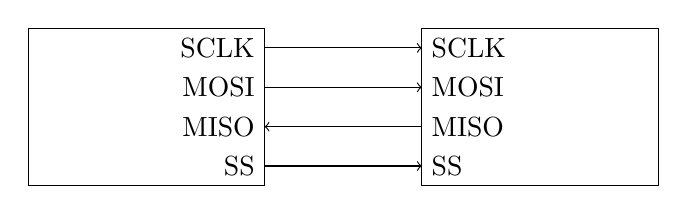
\begin{tikzpicture}
      %% Rectangles.
      \draw[] (0, 0) rectangle (3, 2);
      \draw[] (5, 0) rectangle (8, 2);
      %% Arrows.
      \draw[->] (3, 1.75) -- (5, 1.75);
      \draw[->] (3, 1.25) -- (5, 1.25);
      \draw[<-] (3, 0.75) -- (5, 0.75);
      \draw[->] (3, 0.25) -- (5, 0.25);
      %% Text.
      \node[anchor=east] at (3, 1.75) {SCLK};
      \node[anchor=east] at (3, 1.25) {MOSI};
      \node[anchor=east] at (3, 0.75) {MISO};
      \node[anchor=east] at (3, 0.25) {SS};
      \node[anchor=west] at (5, 1.75) {SCLK};
      \node[anchor=west] at (5, 1.25) {MOSI};
      \node[anchor=west] at (5, 0.75) {MISO};
      \node[anchor=west] at (5, 0.25) {SS};
    \end{tikzpicture}
    \caption{\figureCaption}
    \label{fig:spi-bus}
  \end{figure}
}
